\documentclass[final]{article}


\usepackage{APS360}
\usepackage[utf8]{inputenc} % allow utf-8 input
\usepackage[T1]{fontenc}    % use 8-bit T1 fonts
\usepackage{hyperref}       % hyperlinks
\usepackage{url}            % simple URL typesetting
\usepackage{booktabs}       % professional-quality tables
\usepackage{amsfonts}       % blackboard math symbols
\usepackage{nicefrac}       % compact symbols for 1/2, etc.
\usepackage{microtype}      % microtypography
\usepackage{xcolor}         % colors
 
\title{Project Progress Report for DriveVision}

\author{%
  Naz Saral \\
  1010184408, naz.saral@mail.utoronto.ca,
 \href{}{https://github.com/nazsaral5/project-aps360.git}
\\
}
\usepackage{graphicx}
\begin{document}

\maketitle
\vspace*{-0.5in}
\section*{Project Description}
Traffic sign recognition systems play a fundamental role in developing technologies such as autonomous driving and driving assistance systems used in vehicles today. It is exciting to witness that vehicles today can interpret road rules and respond actively to their environment. This semester I’ll be working on the traffic sign recognition tool called DriveVision. The goal of my project is to design and prototype an image classification tool that will recognize traffic signs around the globe, but specifically evaluated on our very own signs by the Ministry of Transportation (MTO) here in Ontario. I will scope down my project to identify five types of signage; the red and white octagonal Stop sign, the upside down triangular Yield sign, the rectangular and circular Speed Limit sign, the circular No-entry sign, and the rectangular One-way sign. The overall image classification will be done using convolutional neural networks (CNNs) to recognize and classify the five traffic signs. For the speed limit signs especially, I also hope to be able to classify the limit value itself, as this is critical for autonomous driving especially. Model performance is evaluated using classification accuracy and confusion matrices on both the benchmark dataset and the Ontario evaluation dataset.
\begin{figure}[!h]
  \centering
  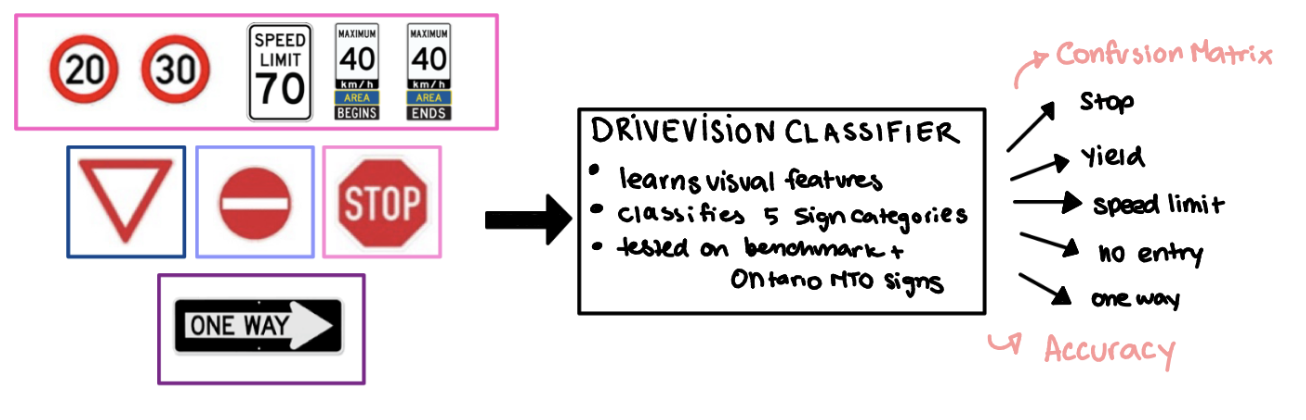
\includegraphics[width=0.8\linewidth]{image1.png}
  \caption{High-level overview of the DriveVision traffic sign recognition blackbox.}
  \label{fig:drivevision}
\end{figure}
\vspace{-0.2in}
\section*{Data Processing}
Upon collecting data from a GTSRB - German Traffic Sign Recognition Benchmark obtained from Kaggle [6]. I started preprocessing the data, as outlined in the proposal. Beginning with selecting the classes containing my 5 signs of focus; 0-8: \texttt{'speed limit'}, 13: \texttt{'yield'}, 14: \texttt{'stop'}, 17: \texttt{'no entry'}, 33-39: \texttt{'one way'}, and labeling them as such. I then proceeded to count and display the number of each type of sign in the data set (Figure 2), before assigning a 70/15/15 split of training, validation and testing that led to a total split of; Train: 15476, Val: 3316, Test: 3317. All images used were transformed with the following sequence of changes. 1. Scaling every image down to 32×32 using Resize(32, 32) effectively standardizes the input dimensions so the CNN always receives the same shape tensor. 2. ToTensor() to convert to tensor with shape [3, 32, 32] and rescale to range [0, 1]. 3. Then applied normalization, using ImageNet mean and standard deviation values, which is standard for RGB channels. In addition to these changes, I additionally implemented, 4. a random rotation of 15 decrees which will be effective especially with stop-signs and its octagonal shape, as well as, 5. colour adjustments to ensure random variation in the data which simulates different lighting conditions like overcast or sunny weather. Processed images were then outputted for show. (Figure 3). 
\begin{figure}[!h]
    \centering
    \begin{minipage}{0.38\linewidth}
        \centering
        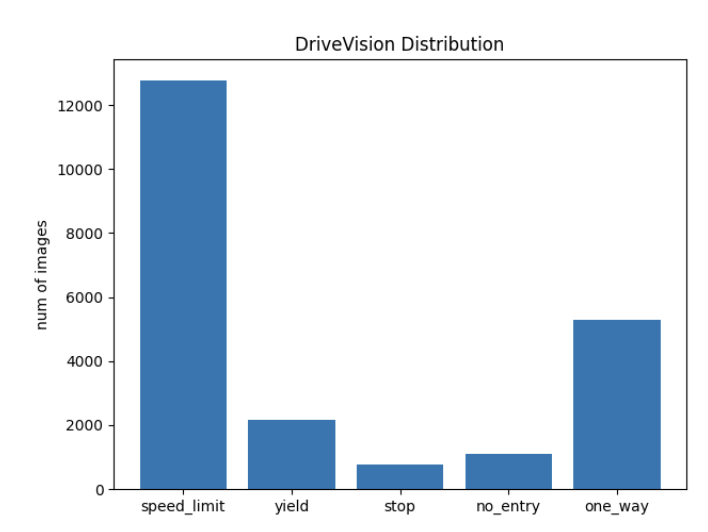
\includegraphics[width=\linewidth]{image2.png}
        \caption{Distribution of classes.}
        \label{fig:image2}
    \end{minipage}
    \hfill
    \begin{minipage}{0.38\linewidth}
        \centering
        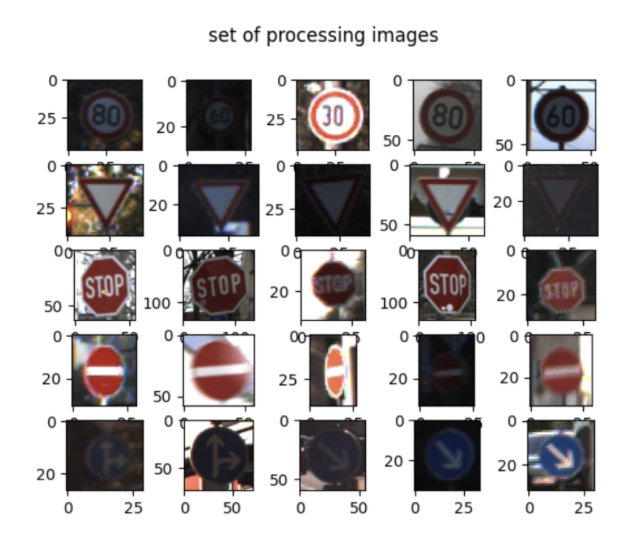
\includegraphics[width=\linewidth]{image3.png}
        \caption{Sample input preprocessed images.}
        \label{fig:image3}
    \end{minipage}
\end{figure}
\newpage
Some challenges presented in this phase show a noticeable class imbalance as the stop has only 780 samples vs. 12,780 for \texttt{'speed limit'}. Passing weights inversely proportional to class frequency into CrossEntropyLoss, so that mistakes on smaller classes are penalized more heavily will help with this challenge. Additionally, with the dataset used, a model trained on one region may not generalize to another. Since I would like this model to be evaluated on Ontario traffic signs, which may differ in fonts, color schemes and layouts. To overcome this, I will add a subset of relevant MTO signs that would be found within the province to strengthen my model's use here in Ontario, to use in my final implementation to ensure adequate model evaluation.
\vspace{-0.1in}
\section*{Baseline Model}
\begin{figure}[!h]
  \centering
  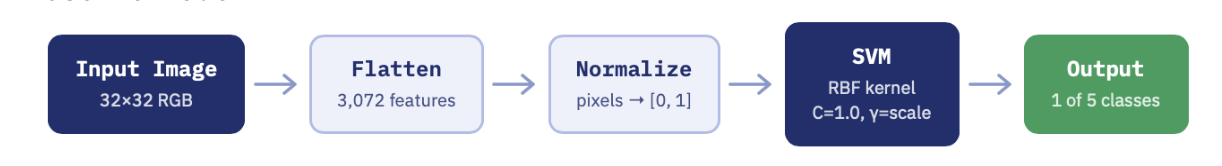
\includegraphics[width=0.8\linewidth]{image4.png}
  \caption{Workflow of SVM Baseline for DriveVision.}
  \label{fig:drivevision}
\end{figure}
The baseline model used is a Support Vector Machine (SVM). The structure of the model as shown in Figure XX, shows no spatial awareness, so just sees a flat list of pixel values. A quantitative measure of the success of this model is a 0.9843 validation accuracy, in addition to this, the confusion matrix below shows that the model performs the best on \texttt{'speed limit'} with 1917 samples being correctly identified. But a common error is that classes are occasionally misclassified as \texttt{'speed limit'}, this can be attributed to the fact it has the most samples. A challenge I faced training this model was a longer than usual runtime, which can be attributed to the large flattened inputs which is computationally expensive (about O(n²) to O(n³)) another issue at hand is that in future renditions, the model cannot generalize to Ontario signs as it is trained on European signs.
\begin{figure}[!h]
  \centering
  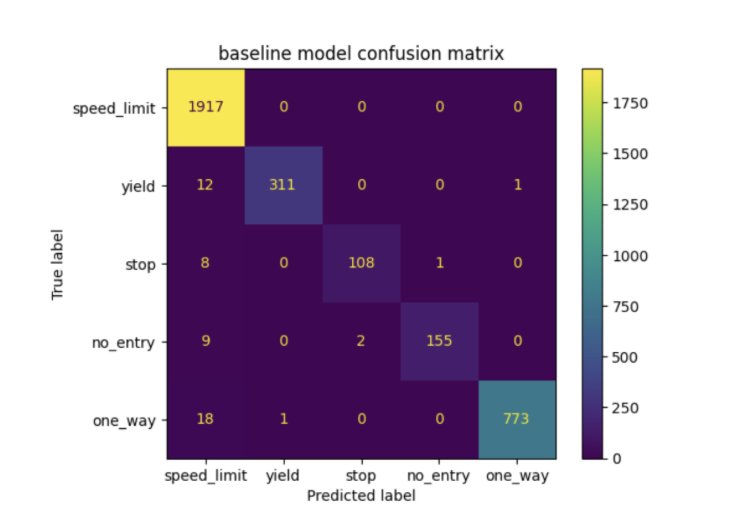
\includegraphics[width=0.5\linewidth]{image5.png}
  \caption{Confusion Matrix for Baseline Model Evaluation.}
  \label{fig:drivevision}
\end{figure}
\vspace{-0.1in}
\newpage
\section*{Primary Model}
\begin{figure}[!h]
  \centering
  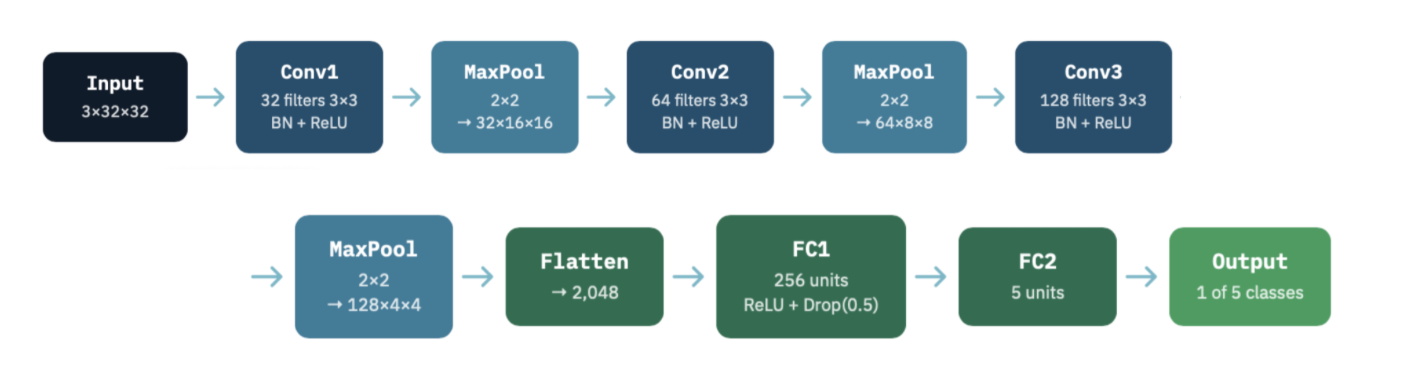
\includegraphics[width=1\linewidth]{image6.png}
  \caption{Workflow of Primary Model (CNN) for DriveVision.}
  \label{fig:drivevision}
\end{figure}
A primary mode as shown in Figure XXl, that emulates what the final CNN will accomplish, is built with 3 convolutional layers, 3 pooling layers that are then flattened and passed through 2 fully connected layers. It contains nearly 620,000 trainable parameters. The validation accuracy of this model is nearly perfect at 0.9993, as observed in the confusion matrix there is minimal error, with only 2/3317 samples of the most prevalent stop-sign class being misclassified. Some challenges that this primary model possesses are that the 32 x 32 resolution is quite low as seen in Figure XX and would pose difficulty in a potential speed limit detection function. Another issue at hand, similar to that of the SVM, is that I have yet to include data from local Ontario MTO signage, which I hope to implement in the final model, for training and evaluation.
\begin{figure}[!h]
    \centering
    \begin{minipage}{0.4\linewidth}
        \centering
        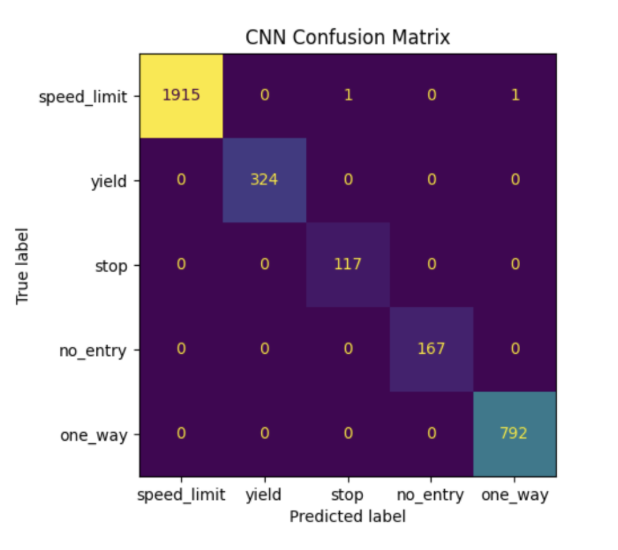
\includegraphics[width=\linewidth]{image7.png}
        \caption{Confusion Matrix for Primary Model Evaluation.}
        \label{fig:image2}
    \end{minipage}
    \hfill
    \begin{minipage}{0.44\linewidth}
        \centering
        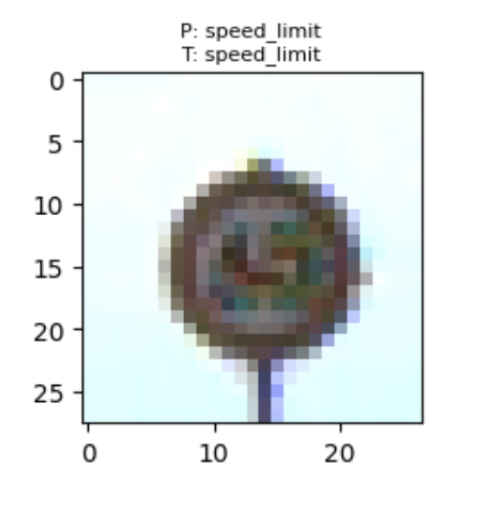
\includegraphics[width=\linewidth]{image8.png}
        \caption{Sample 32 by 32 Input Image (BLURRY).}
        \label{fig:image3}
    \end{minipage}
\end{figure}
\newpage
\section*{References}

[1] @inproceedings{ren2009traffic,
  author    = {Ren, Fei-Xiang and Huang, Jinsheng and Jiang, Ruyi and Klette, Reinhard},
  title     = {General Traffic Sign Recognition by Feature Matching},
  booktitle = {Proceedings of the 24th International Conference on Image and Vision Computing New Zealand},
  pages     = {409--414},
  year      = {2009},
  doi       = {10.1109/IVCNZ.2009.5378370}
}

[2] @article{cao2019traffic,
  title   = {Improved Traffic Sign Detection and Recognition Algorithm for Intelligent Vehicles},
  author  = {Cao, J. and Song, C. and Peng, S. and Xiao, F. and Song, S.},
  journal = {Sensors},
  volume  = {19},
  number  = {18},
  pages   = {4021},
  year    = {2019},
  doi     = {10.3390/s19184021}
}

[3] @online{bbc2020tesla,
  title        = {Tesla Updates Autopilot to Read Speed Signs},
  author       = {{BBC News}},
  organization = {BBC},
  year         = {2020},
  url          = {https://www.bbc.com/news/technology-53973511}
}

[4] @online{waymo2020perception,
  title        = {How Waymo Builds a Generalizable Perception System},
  author       = {{Waymo}},
  organization = {Waymo},
  year         = {2020},
  url          = {https://waymo.com/blog/2020/02/content-search}
}

[5] @online{googlemaps2020speedlimits,
  title        = {How AI and Imagery Keep Speed Limits on Google Maps Updated},
  author       = {{Google Maps}},
  organization = {Google},
  year         = {2020},
  url          = {https://blog.google/products-and-platforms/products/maps/how-ai-and-imagery-keep-speed-limits-on-google-maps-updated/}
}

[6] @misc{gtsrbkaggle,
  title        = {GTSRB German Traffic Sign},
  author       = {Meowmeowmeowmeowmeow},
  url = {https://www.kaggle.com/datasets/meowmeowmeowmeowmeow/gtsrb-german-traffic-sign}
}



\end{document}